%        File: arfc-beamer.tex
%     Created: Sun May 5 10:00 PM 2013 C


%\documentclass[11pt,handout]{beamer}
\documentclass[9pt]{beamer}
\usetheme[white]{Illinois}
%\title[short title]{long title}
\title[Research Summary]{Research Activities in the ARFC Group}
%\subtitle[short subtitle]{long subtitle}
\subtitle[Brief Summary]{A Brief Summary}
%\author[short name]{long name}
\author[ARFC]{Advanced Reactors and Fuel Cycles Group}
%\date[short date]{long date}
\date[09.05.2019]{September 5, 2019}
%\institution[short name]{long name}
\institute[UIUC]{University of Illinois at Urbana-Champaign}

%\usepackage{bbding}
\usepackage{amsfonts}
\usepackage{amsmath}
\usepackage{xspace}
\usepackage{graphicx}
\usepackage{subfigure}
\usepackage{booktabs} % nice rules for tables
\usepackage{microtype} % if using PDF
\usepackage{bigints}
\usepackage{minted}
\usepackage[absolute,overlay]{textpos}
\usepackage{tikz}
\usetikzlibrary{positioning, arrows, decorations, shapes}
\usetikzlibrary{shapes.geometric,arrows}
\definecolor{illiniblue}{HTML}{B1C6E2}
\tikzstyle{bblock} = [rectangle, draw, fill=illiniblue, 
text width=10em, text centered, rounded corners, minimum height=4em]
\tikzstyle{sbblock} = [rectangle, draw, fill=illiniblue, 
text width=7em, text centered, rounded corners, minimum height=4em]
\tikzstyle{arrow} = [thick,->,>=stealth]

\newcommand{\units}[1] {\:\text{#1}}%
\newcommand{\SN}{S$_N$}%{S$_\text{N}$}%{$S_N$}%
\DeclareMathOperator{\erf}{erf}
%I need some complimentary error funcitons... 
\DeclareMathOperator{\erfc}{erfc}
%Those icons in the references are terrible looking
\setbeamertemplate{bibliography item}[text]

%%%% Acronym support

\usepackage[acronym,toc]{glossaries}
\include{acros}

\makeglossaries

%try to get rid of header on title page\dots
\makeatletter
    \newenvironment{withoutheadline}{
        \setbeamertemplate{headline}[default]
        \def\beamer@entrycode{\vspace*{-\headheight}}
    }{}
\makeatother

\makeatother
\setbeamertemplate{footline}
{
  \leavevmode%
  \hbox{%
    \rightline{\insertframenumber{} / \inserttotalframenumber\hspace*{1ex}}
  }%
  \vskip0pt%
}
\makeatletter
\begin{document}
%%%%%%%%%%%%%%%%%%%%%%%%%%%%%%%%%%%%%%%%%%%%%%%%%%%%%%%%%%%%%
%% From uw-beamer Here's a handy bit of code to place at 
%% the beginning of your presentation (after \begin{document}):
\newcommand*{\alphabet}{ABCDEFGHIJKLMNOPQRSTUVWXYZabcdefghijklmnopqrstuvwxyz}
\newlength{\highlightheight}
\newlength{\highlightdepth}
\newlength{\highlightmargin}
\setlength{\highlightmargin}{2pt}
\settoheight{\highlightheight}{\alphabet}
\settodepth{\highlightdepth}{\alphabet}
\addtolength{\highlightheight}{\highlightmargin}
\addtolength{\highlightdepth}{\highlightmargin}
\addtolength{\highlightheight}{\highlightdepth}
\newcommand*{\Highlight}{\rlap{\textcolor{HighlightBackground}{\rule[-\highlightdepth]{\linewidth}{\highlightheight}}}}
%%%%%%%%%%%%%%%%%%%%%%%%%%%%%%%%%%%%%%%%%%%%%%%%%%%%%%%%%%%%%
%%--------------------------------%%
\begin{withoutheadline}
\frame{
  \titlepage
}
\end{withoutheadline}

%%--------------------------------%%
\AtBeginSection[]{
\begin{frame}
  \frametitle{Outline}
  \tableofcontents[currentsection]
\end{frame}
}

\section{Software}
\input{cyclus}
\input{moltres}
\begin{frame}
\frametitle{SaltProc flowchart}
\vspace{-2mm}
\begin{figure}[ht!] % replace 't' with 'b' to \centering
	\centering
	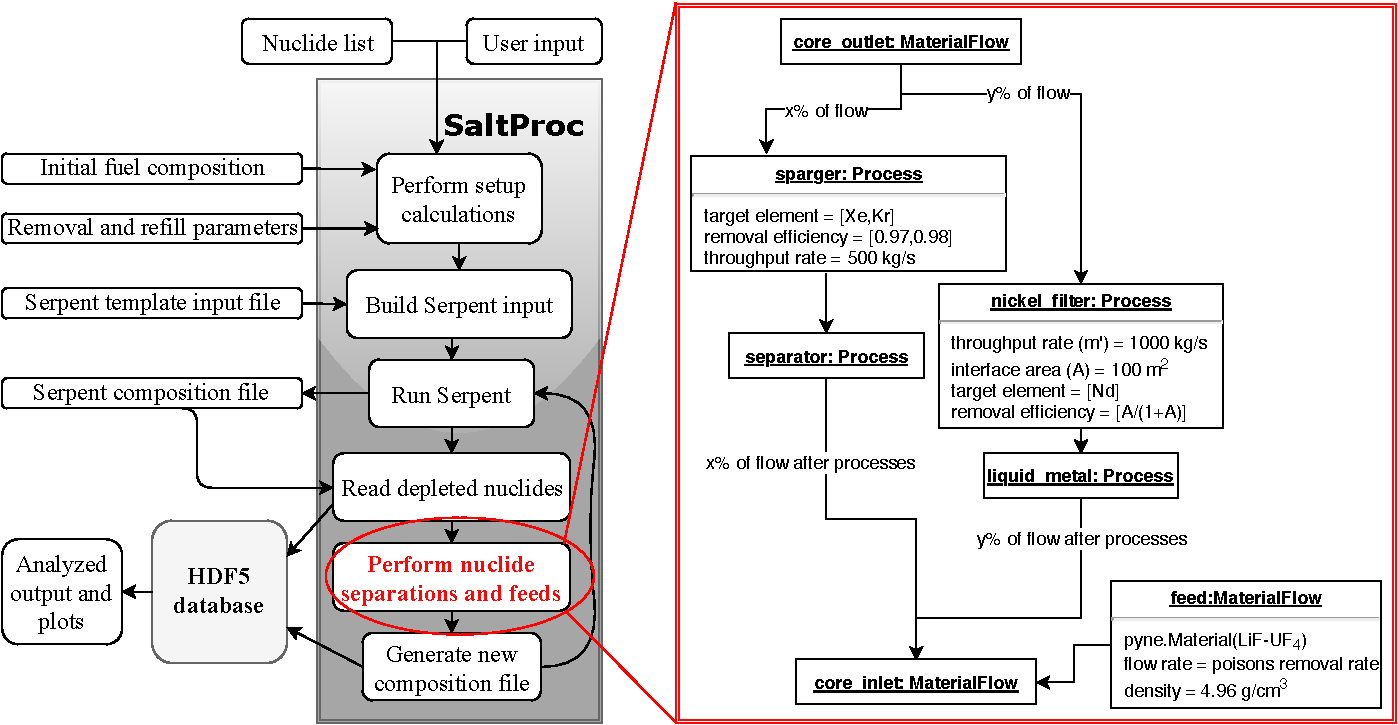
\includegraphics[width=1.05\textwidth]{./images/saltproc_flowchart.pdf}
	\caption{Tentative generic flowchart for SaltProc v1.0 python package.}
\end{figure}

\end{frame}
\input{annsa}
% needed to create images without issue
\graphicspath{{./images/}}

	\begin{frame}
		\frametitle{\texttt{ANNSA}}
		``$\textbf{A}$rtificial $\textbf{N}$eural $\textbf{N}$etworks for $\textbf{S}$pectroscopic $\textbf{A}$nalysis"\\
		\begin{enumerate}
			\item Isotopics
			\item Nuclear Verification
			\item National Security 
			\item Machine Learning
		\end{enumerate}
	\end{frame}	
	\begin{frame}
		\frametitle{$\texttt{ANNSA}$}
		\begin{enumerate}
			\item Motivation\\
			Improve upon the current spectroscopy workflow
			\item Method\\
			Convolutional Neural Networks
		\end{enumerate} 
	\end{frame}
	% image frame
	\begin{frame}
		\frametitle{$\texttt{ANNSA}$ - Convolutional Neural Network}
		\begin{figure}
			\includegraphics[width=4cm]{cnn-figure.png}
			\caption{A 1-D CNN with a gamma ray spectrum as input. Credit: Mark Kamuda}
		\end{figure}
	\end{frame}

	\begin{frame}
		\frametitle{$\texttt{ANNSA}$ - Extensions and Future Work}
		\begin{enumerate}
			\item Algorithm Improvements
			\item Different Detectors
			\item More complicated isotopics
		\end{enumerate}
	\end{frame}


	\begin{frame}
		\frametitle{\texttt{CAIRO}}
		``$\textbf{C}$omputerized $\textbf{A}$rtificially $\textbf{I}$ntelligent $\textbf{R}$eactor $\textbf{O}$perator"\\
		\begin{enumerate}
			\item Nuclear Power
			\item Reactor Controls
			\item Control Room Simulation
			\item Artificial Intelligence
		\end{enumerate}
	\end{frame}

	\begin{frame}
		\frametitle{CAIRO - Motivation}
		\begin{figure}
			\includegraphics[width=5cm]{homer-reactor.jpg}
		\end{figure}
	\end{frame}
	\begin{frame}
		\frametitle{CAIRO - Current Work}
		\begin{enumerate}
			\item Microreactor control room simulator
			\begin{enumerate}
				\item Core
				\item Thermal Power Plant
				\item Control room interface
			\end{enumerate}
			\item Best representation of nuclear power plant for a deep reinforcement learning agent?
			\item What is an appropriate reward function(s) for a deep RL agent?
			\item Much more... 
		\end{enumerate}
	\end{frame}



% \end{document}

\section{Advanced Reactors}
\input{park}
\input{chaube}
\begin{frame}
\frametitle{Transatomic Power (TAP) concept high-fidelity Serpent model}
	  \begin{textblock*}{12.25cm}(0.25cm,1.8cm) % {block width} (coords)
\begin{figure}[htp!] % replace 't' with 'b' to 
	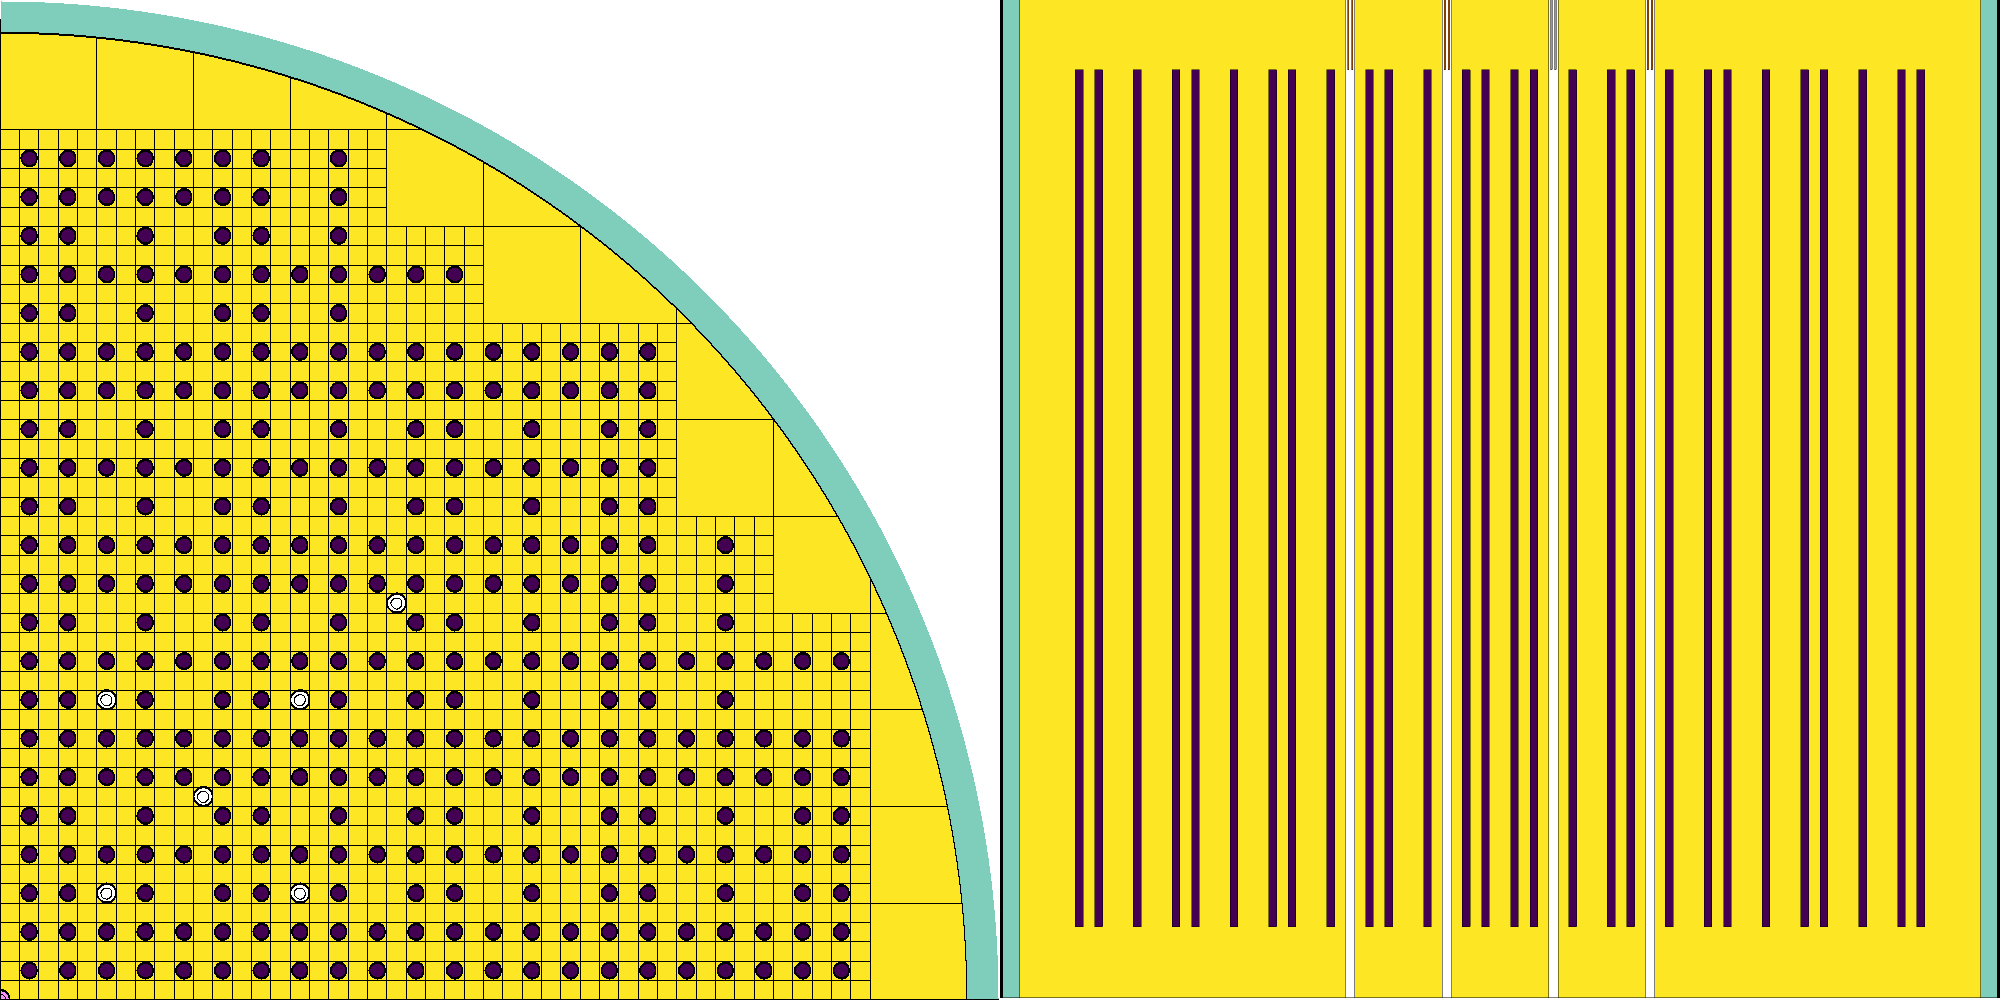
\includegraphics[width=\textwidth]{./images/tap_model.png}
	\caption{An $XY$ (left) and $XZ$ (right) section of the TAP model. 
	The violet color represents zirconium hydride, and the yellow represents 
	fuel salt (reproduced from Rykhlevskii \& Huff, Milestone 2.1 Report, 
	2019).}
\end{figure}
	  \end{textblock*}
\end{frame}


\begin{frame}
\frametitle{Depletion simulation results for TAP with various feeds}       
\begin{textblock*}{12.6cm}(0.1cm,2.2cm) % {block width} (coords)
	\begin{figure}[htp!] % replace 't' with 'b' to 
		\begin{minipage}[b]{0.48\textwidth}
			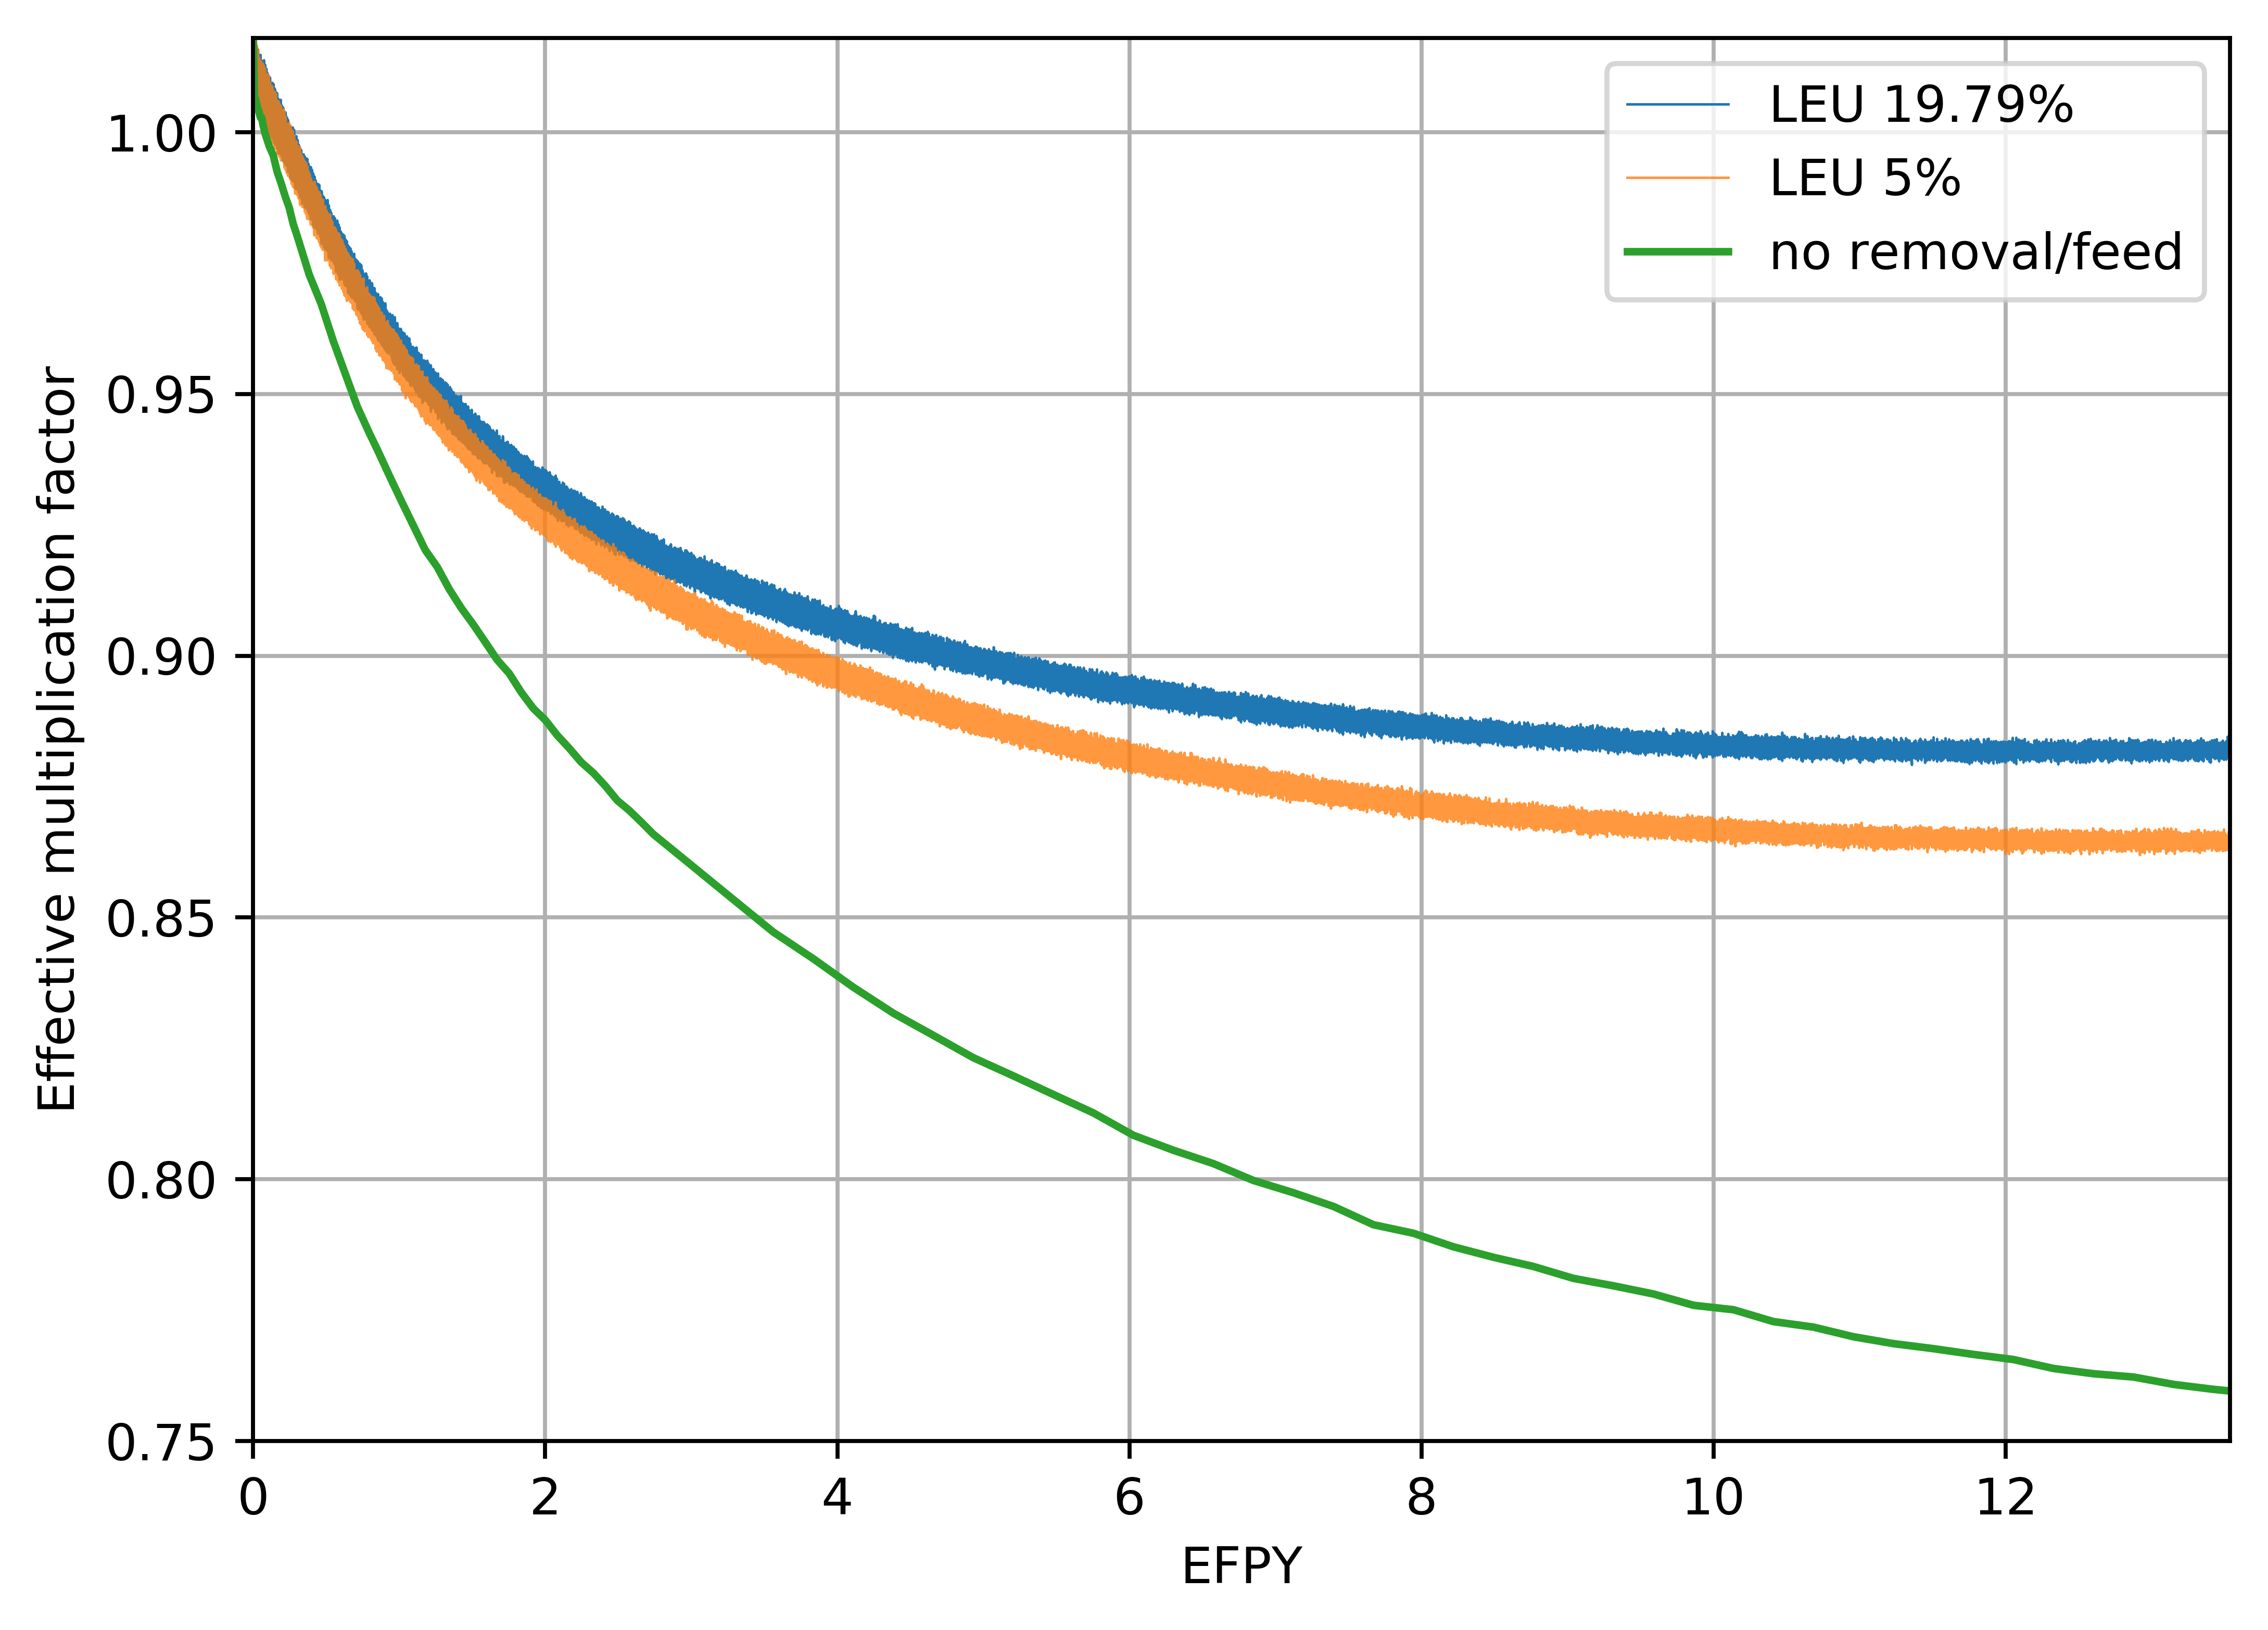
\includegraphics[width=\linewidth]{./images/keff_3.png}
		\end{minipage}
			\hspace{-2mm}
		\begin{minipage}[b]{0.48\textwidth}
			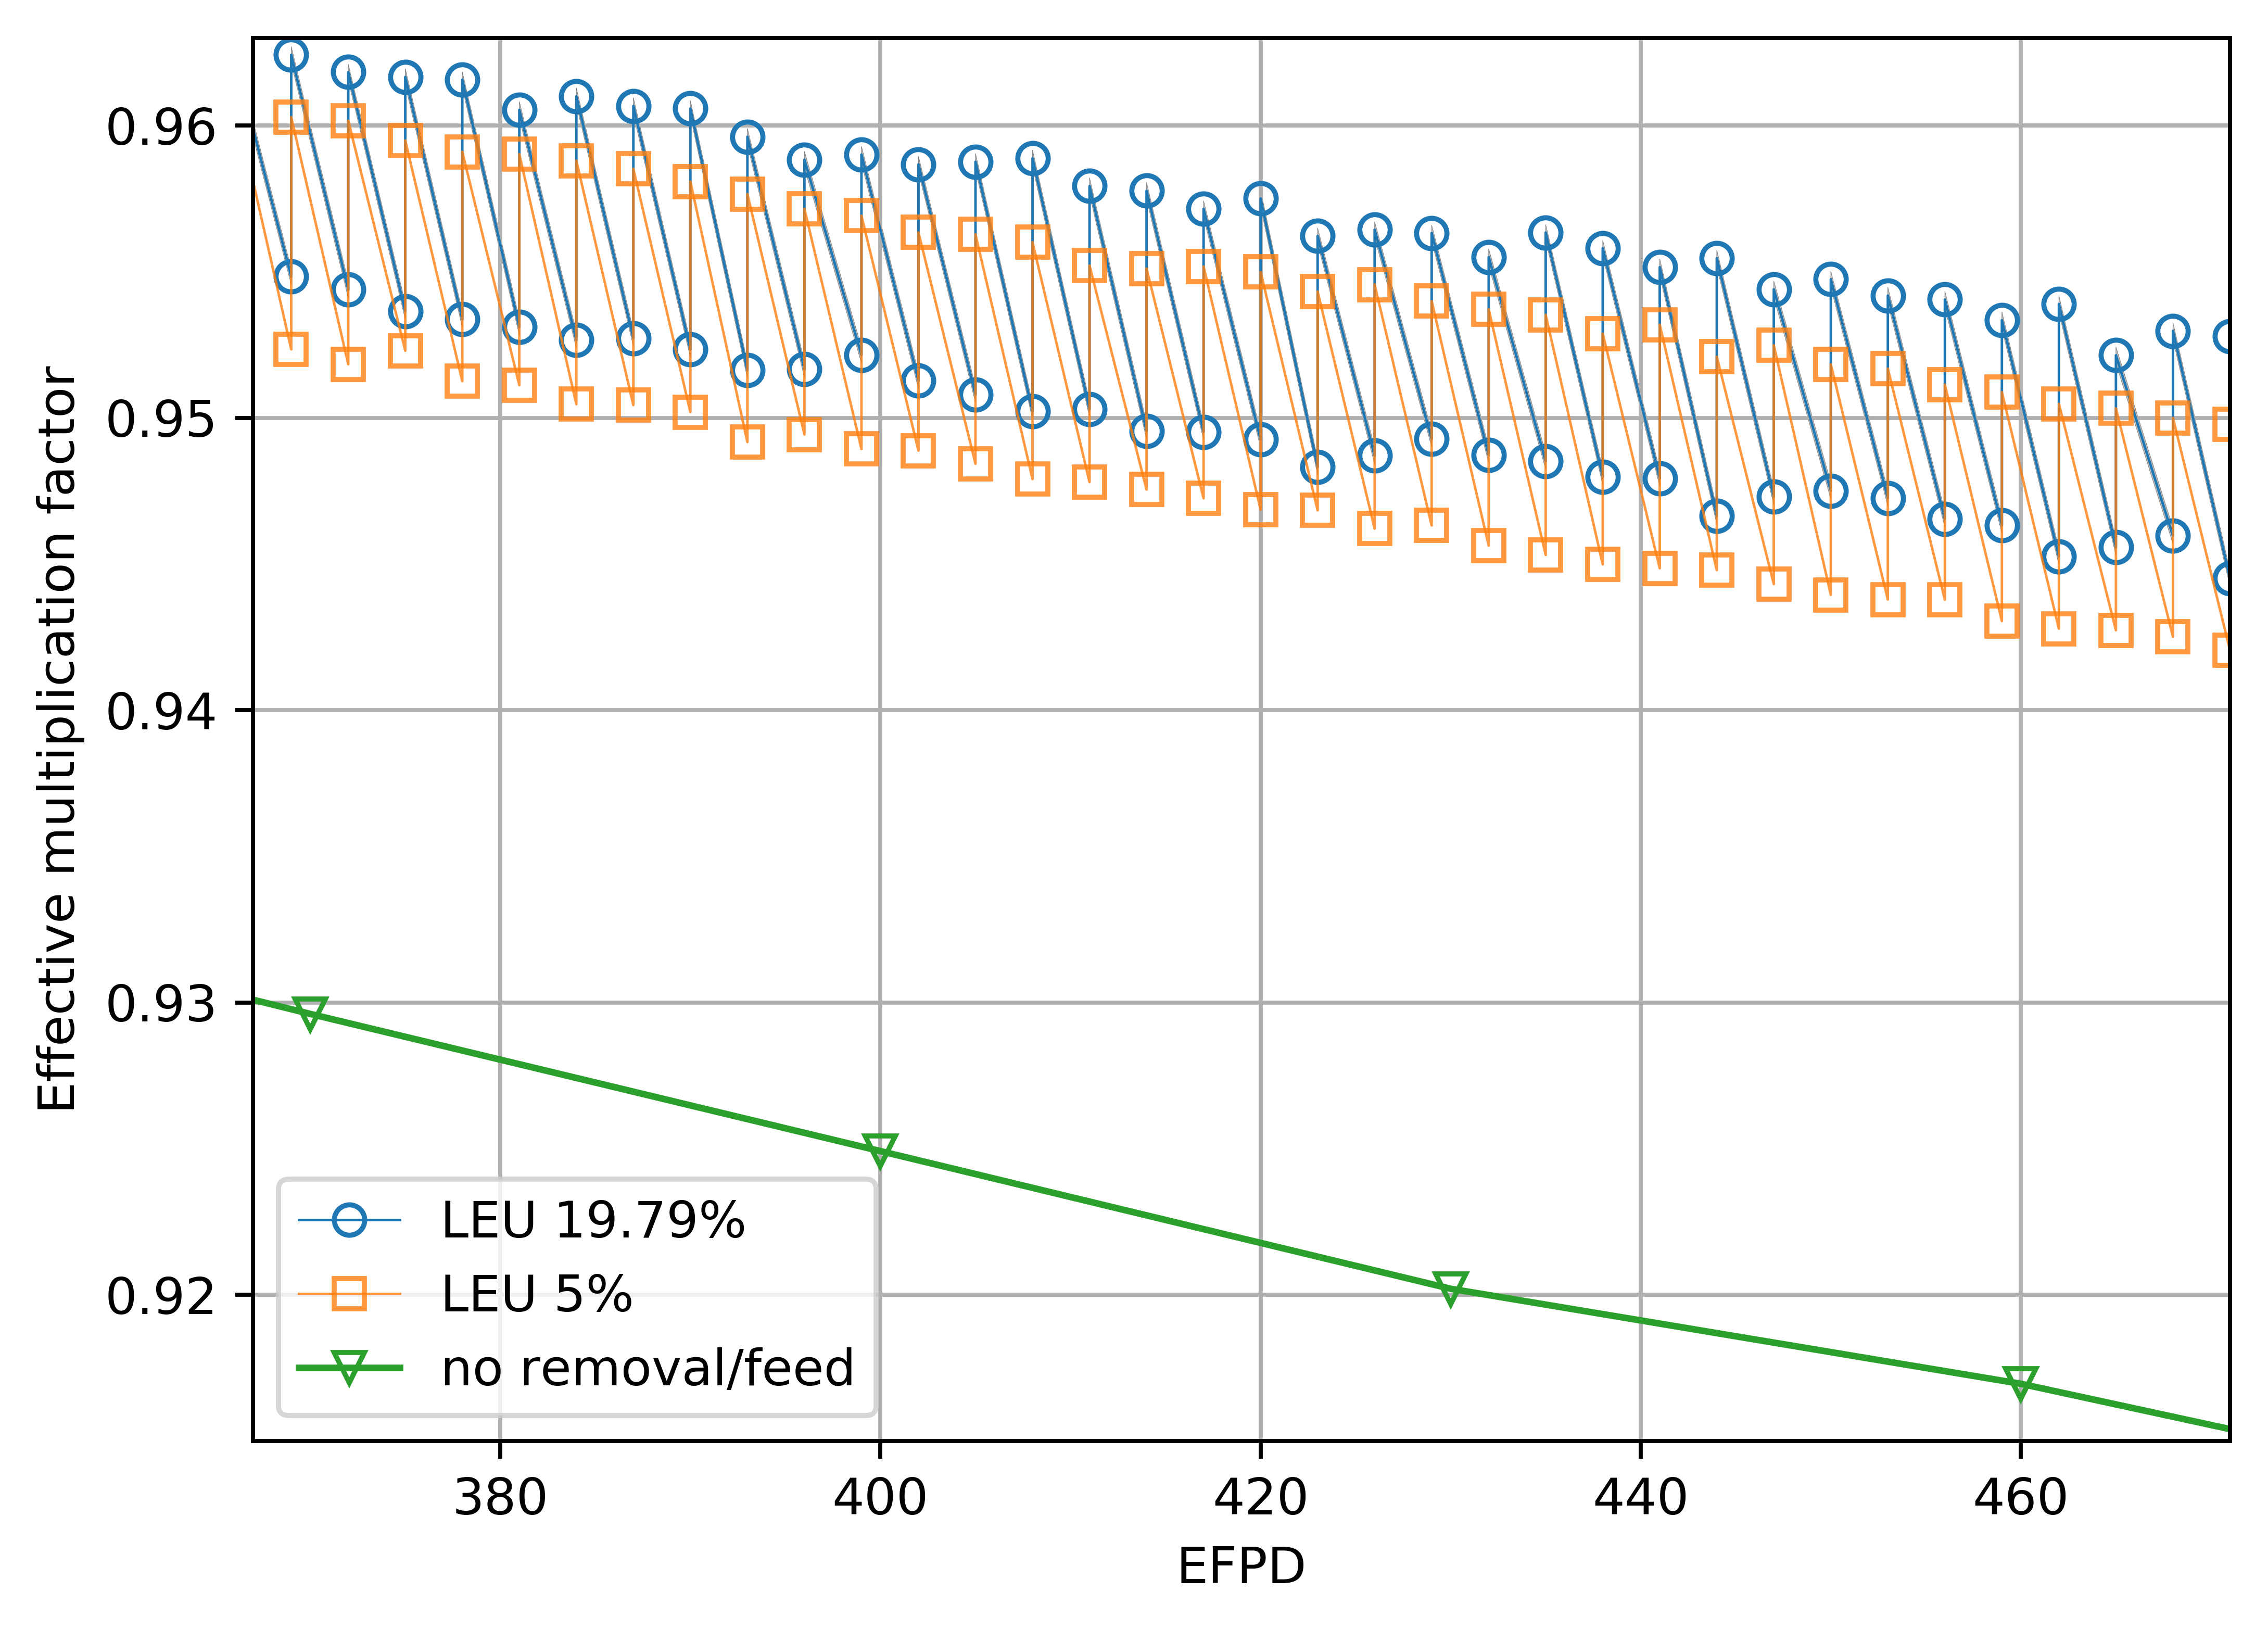
\includegraphics[width=\linewidth]{./images/keff_zoomed_2.png}
		\end{minipage}
		\caption{Effective multiplication factor dynamics for full-core
		TAP model for different fueling scenarios over a 13-year reactor 
		operation (left) and for the time interval from 367 to 471 days after 
		startup (right). Confidence interval $\pm\sigma=28pcm$ is shaded.}
	\end{figure}
\end{textblock*}
\end{frame}


\begin{frame}
\frametitle{Fuel salt composition evolution during the TAP operation}
\begin{textblock*}{12.25cm}(0.25cm,2cm) % {block width} (coords)
	\begin{figure}[htp!] % replace 't' with 'b' to 
		\centering
				\vspace{-3mm}
		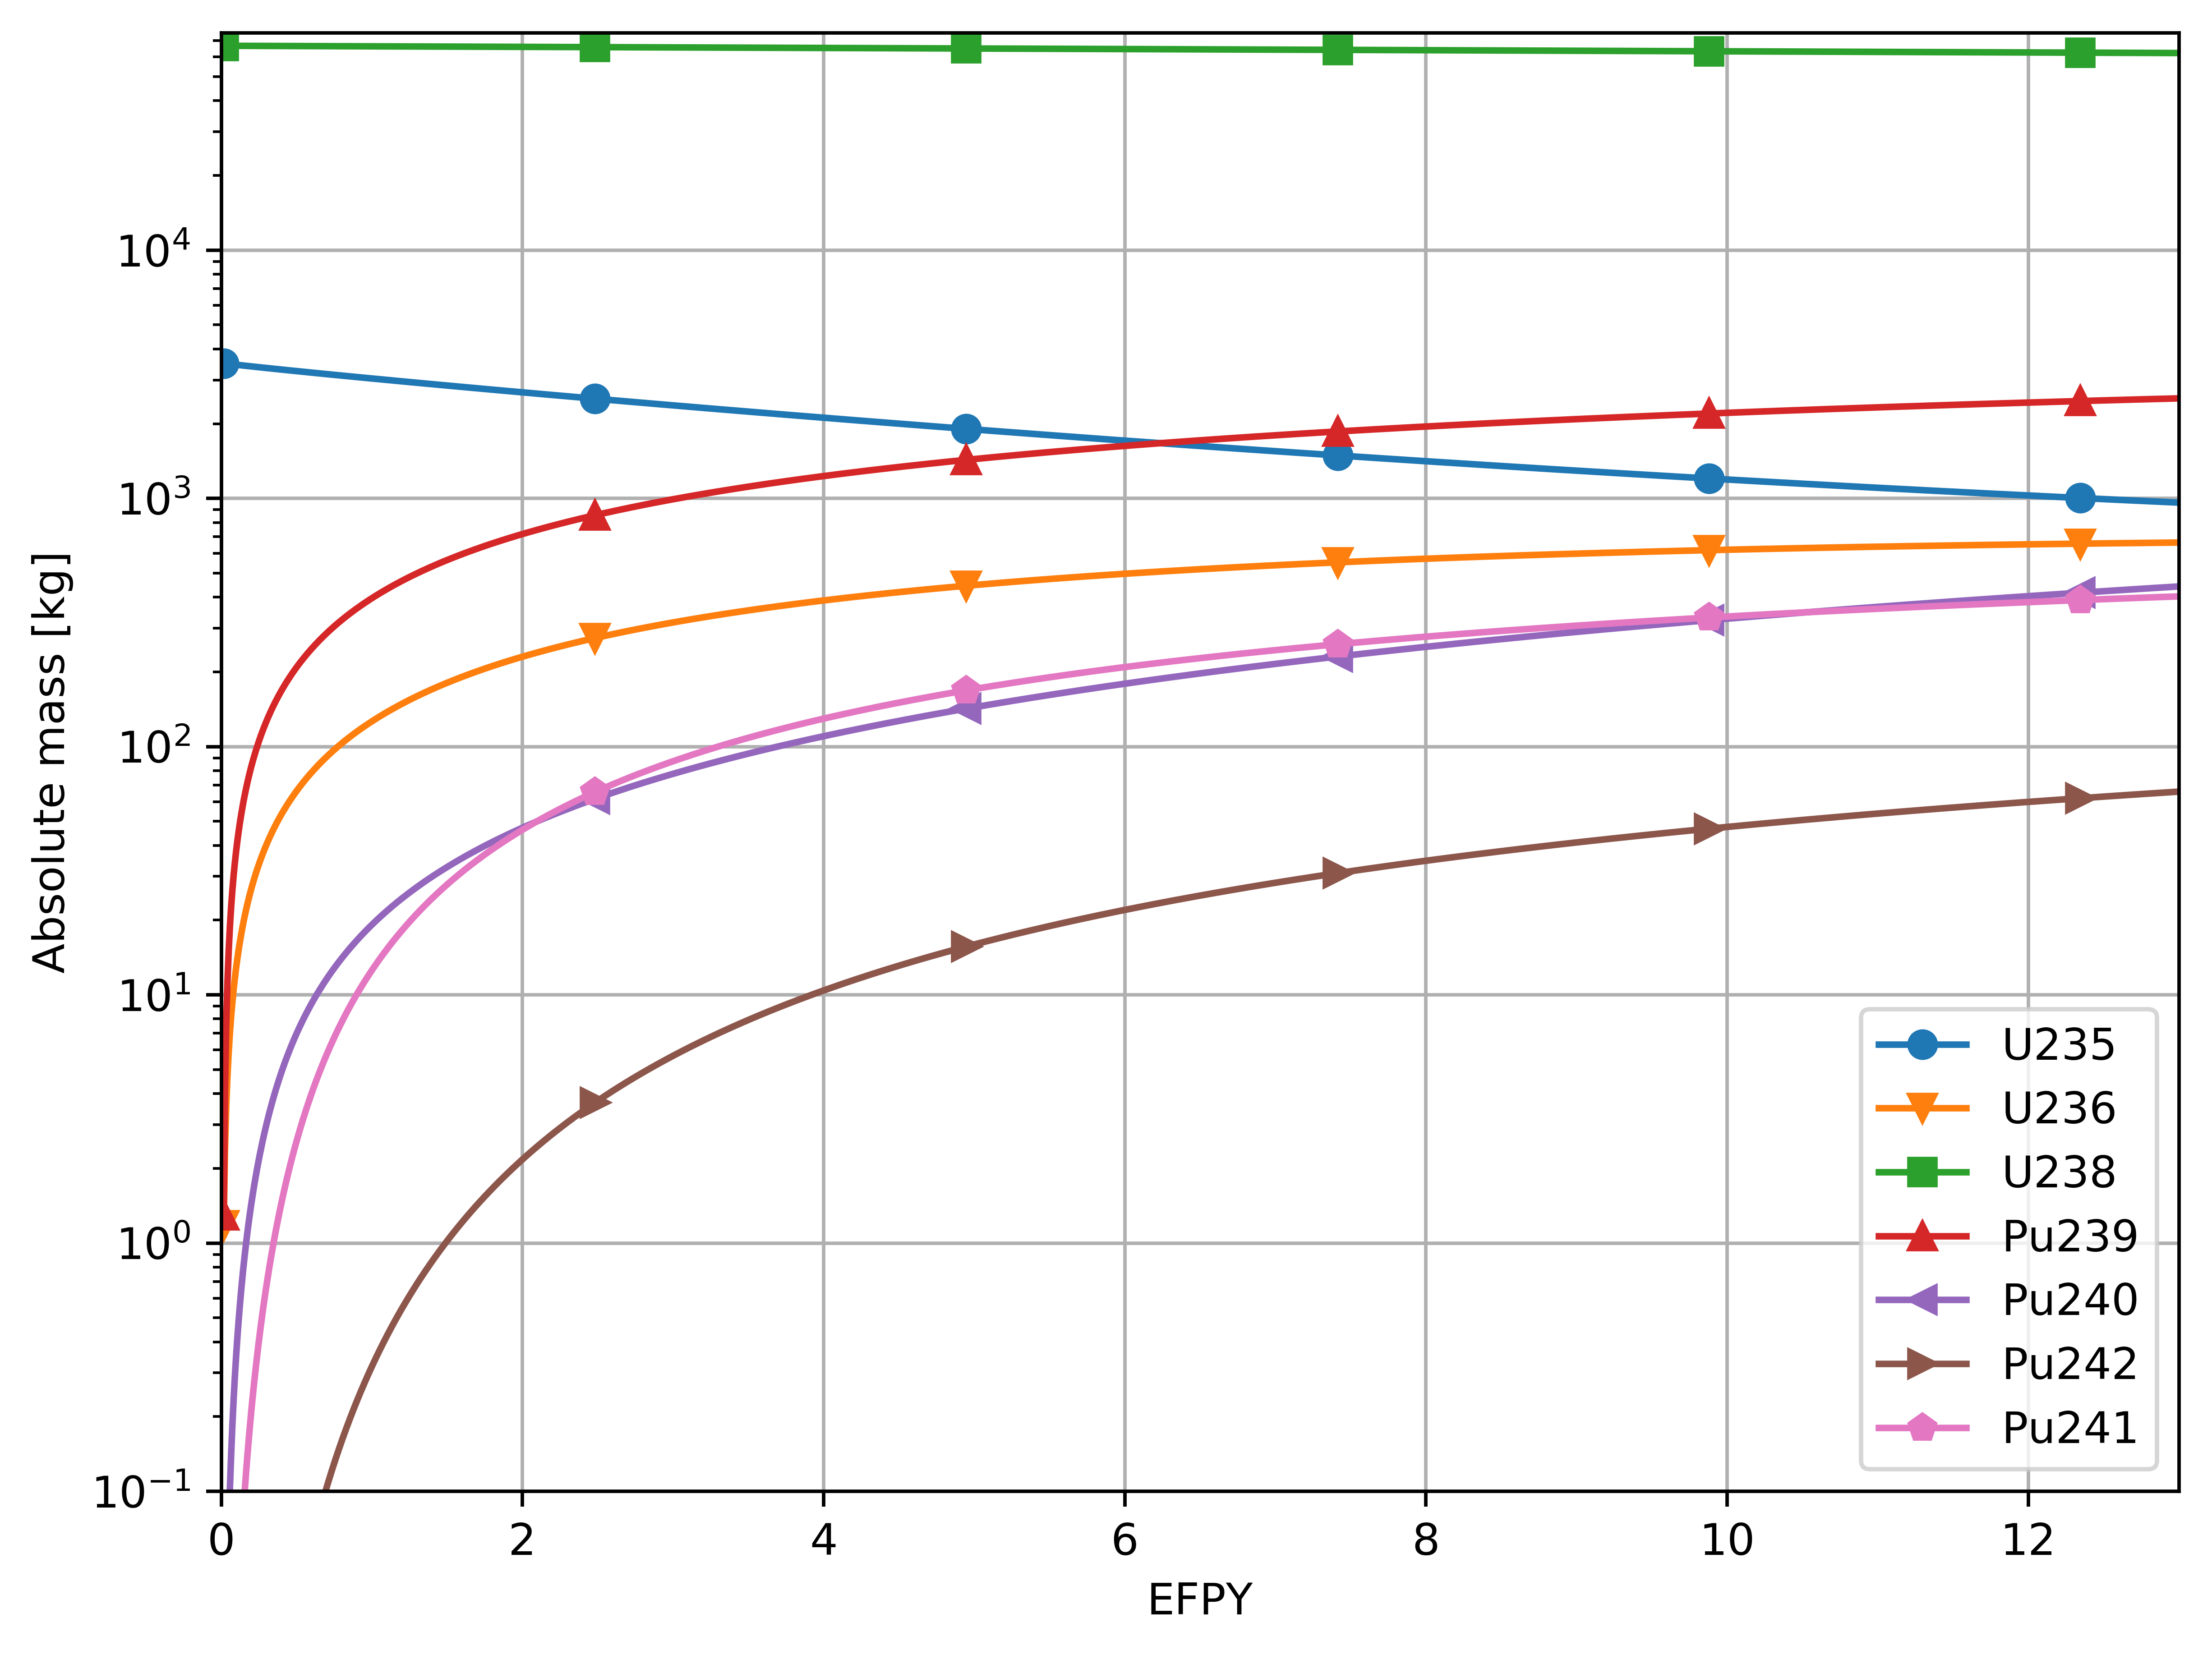
\includegraphics[width=0.72\textwidth]{../images/u_pu_mass.png}
		\caption{Mass of major nuclides during 13 years of reactor operation 
		with 19.79\% low-enriched uranium feed.}
	\end{figure}
\end{textblock*}
\end{frame}
\begin{frame}
\frametitle{Microreactors: Motivation}
\begin{columns}
  \column[t]{5cm}
  Microreactors can fulfill energy needs in special use cases, or in
  areas with a greater population.
  \column[t]{5cm}
    \begin{figure}[htbp!]
    \begin{center}
    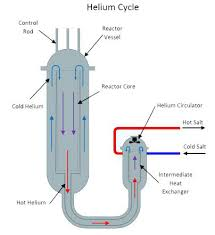
\includegraphics[height=4cm]{./images/mmr-chalk-river}
    \end{center}
    \caption{A Diagram of the proposed MMR for the Chalk River project. \cite{mmr-chalk-river}.}
    \label{fig:mmr-chalk-river}
    \end{figure}

\end{columns}
\end{frame}


\begin{frame}
\frametitle{Siting Considerations for Microreactors}

  \begin{itemize}
    \item Current guidelines based on LWRS
    \item Experience tells us radionuclide release is not as severe as once feared.
  \end{itemize}

  The first step in these revised siting considerations is to determine a source term.

\end{frame}

\input{fairhurst1}
\section{Fuel Cycles}
\input{westphal}
\input{chee}
\input{fairhurst2}

\section{Acknowledgments}
\begin{frame}
  \frametitle{Acknowledgments}
        
	Zoe Richter is currently funded by an NRC fellowship, and would like to thank Dr. Huff, 	Andrei Rykhlevskii, Roberto Fairhurst, and Sam Dotson of the ARFC team at UIUC.

	Acknowledgements should include both people who helped and funding 
        streams. If you are funded by an NEUP grant, that number usually goes 
        here. .
\end{frame}

%%--------------------------------%%
%%--------------------------------%%
\begin{frame}[allowframebreaks]
  \frametitle{References}
  \bibliographystyle{plain}
  {\footnotesize \bibliography{2019-09-05-group.bib} }
\end{frame}

%%--------------------------------%%

% Examples 
% ARFC Team: Some good examples of how to use beamer are in this file.
% You can use this to guide the preparation of slides.
\input{example}


\end{document}

